\documentclass{article}
\usepackage{a4wide}
\usepackage{graphicx}
\usepackage{amsmath, amsthm, amssymb}

\usepackage[utf8]{inputenc}
\usepackage{ngerman}
\usepackage{url}
\usepackage[ruled,vlined]{algorithm2e}
\usepackage[]{hyperref}
\usepackage{listings}
\usepackage{dsfont}

\newtheorem{thm}{Theorem}[section]
\newtheorem{cor}[thm]{Korollar}
\newtheorem{lem}[thm]{Lemma}
\newtheorem{defi}[thm]{Definition}
\newtheorem{definition}{Definition}
\newcounter{Chapcounter}
\newcommand\showmycounter{\addtocounter{Chapcounter}{1}\themycounter}
\newcommand{\chapter}[1] 
{ {\centering          
  \addtocounter{Chapcounter}{1} \Large \underline{\textbf{ \color{blue} Chapter \theChapcounter: ~#1}} }   
  \addcontentsline{toc}{section}{ \color{blue} Chapter:~\theChapcounter~~ #1}    
}
\hypersetup{colorlinks=true}
\hypersetup{linkcolor=black}
\usepackage{listings}
\lstdefinelanguage{Pseudo}{
  morekeywords={forall,if,then,else,return,while,do,for,DFS},
  sensitive=false,
  morecomment=[l]{//},
  morestring=[b]"
}



\setcounter{tocdepth}{4}

\begin{document}

% ============================================================================
% Title Page
% ============================================================================
\title{Formulas for Statistische und Stochastische Grundlagen der Informatik}
\date{Wintersemester 2025/26}
\author{Universität Stuttgart}
\maketitle

\tableofcontents
\newpage

% ============================================================================
% Chapter 1: Stochastic
% ============================================================================
\chapter{Stochastic}

% ----------------------------------------------------------------------------
\section{Finite Probability Space}
% ----------------------------------------------------------------------------

A finite probability space is defined as a tuple:
\[
    (\Omega, \mathbb{P}) \quad \text{where} \quad 0 < |\Omega| < \infty
\]
with the probability measure:
\[
    \mathbb{P} : \mathcal{P}(\Omega) \to \mathbb{R}
\]

\subsection{Axioms of Probability}

The probability measure $\mathbb{P}$ satisfies the following properties:

\begin{enumerate}
    \item \textbf{Non-negativity:} 
    \[
        \forall A \subseteq \Omega : \mathbb{P}(A) \geq 0
    \]
    
    \item \textbf{Normalization:} 
    \[
        \mathbb{P}(\Omega) = 1
    \]
    
    \item \textbf{Additivity for disjoint events:} 
    \[
        \forall A, B \subseteq \Omega, \, A \cap B = \emptyset : \mathbb{P}(A \cup B) = \mathbb{P}(A) + \mathbb{P}(B)
    \]
\end{enumerate}

\noindent
\textit{Note:} All other properties of probability can be derived from these axioms.

% ----------------------------------------------------------------------------
\section{Random Variables}
% ----------------------------------------------------------------------------

A \textbf{random variable} is a function:
\[
    X : \Omega \to \mathbb{R}
\]
that tracks a particular property of the probability space.

\medskip
\noindent
A \textbf{distribution function} describes the probability of each value of the random variable. The cumulative distribution function follows trivially.

% ----------------------------------------------------------------------------
\section{Special Concepts}
% ----------------------------------------------------------------------------

\subsection{Laplace Experiment}
In a Laplace experiment, all elementary events have equal probability.

\subsection{Indicator Function}
The indicator function for a set $A$ is defined as:
\[
    \mathbb{1}_A(x) = 
    \begin{cases}
        1 & \text{if } x \in A \\
        0 & \text{if } x \notin A
    \end{cases}
\]

% ----------------------------------------------------------------------------
\section{Expected Value}
% ----------------------------------------------------------------------------

The \textbf{expected value} of a random variable $X$ represents its average value:
\[
    \mathbb{E}(X) := \sum_{w \in \Omega} X(w) \, \mathbb{P}(\{w\}) 
    = \sum_{x \in X(\Omega)} x \cdot \mathbb{P}(X = x)
\]

\subsection{Properties of Expected Value}

\begin{enumerate}
    \item \textbf{Linearity:}
    \[
        \mathbb{E}\left(\sum_{i=1}^n \alpha_i X_i\right) = \sum_{i=1}^n \alpha_i \, \mathbb{E}(X_i)
    \]
    
    \item \textbf{Expected value of indicator function:}
    \[
        \mathbb{E}(\mathbb{1}_A) = \mathbb{P}(A)
    \]
\end{enumerate}

% ----------------------------------------------------------------------------
\section{Variance and Standard Deviation}
% ----------------------------------------------------------------------------

The \textbf{variance} measures the spread of a random variable's distribution (higher variance indicates greater spread):
\[
    \mathbb{V}(X) := \mathbb{E}\left((X - \mathbb{E}(X))^2\right) = \mathbb{E}(X^2) - \mathbb{E}(X)^2
\]

\subsection{Properties of Variance}

For constants $a, b \in \mathbb{R}$:
\[
    \mathbb{V}(aX + b) = a^2 \, \mathbb{V}(X)
\]

\subsection{Standard Deviation}

The \textbf{standard deviation} is defined as:
\[
    \sigma(X) := \sqrt{\mathbb{V}(X)}
\]

% ----------------------------------------------------------------------------
\section{Chebyshev's Inequality}
% ----------------------------------------------------------------------------

Chebyshev's inequality provides a conservative bound on the probability of deviation from the expected value:
\[
    \mathbb{P}\left(|X - \mathbb{E}(X)| \geq \epsilon\right) \leq \frac{\mathbb{V}(X)}{\epsilon^2}
\]

\subsection{Intuition}

\begin{itemize}
    \item Higher variance implies larger possible bounds, as a more spread-out distribution increases the likelihood of values lying outside a given range.
    \item The bound is inversely proportional to $\epsilon^2$: increasing the tolerance $\epsilon$ decreases the probability of exceeding it.
\end{itemize}

% ----------------------------------------------------------------------------
\section{Independence}
% ----------------------------------------------------------------------------

\subsection{Independence of Events}

Two events $A$ and $B$ are \textbf{independent} if:
\[
    \mathbb{P}(A \cap B) = \mathbb{P}(A) \cdot \mathbb{P}(B)
\]

\subsection{Independence of Random Variables}

Random variables $X_1, \ldots, X_n$ are \textbf{independent} if for all sets $B_1, \ldots, B_n$:
\[
    \mathbb{P}(X_1 \in B_1, \ldots, X_n \in B_n) = \prod_{i=1}^n \mathbb{P}(X_i \in B_i)
\]
\subsection{Application of independent random variables}
For independent random variables
\[\mathbb{E}(X\cdot Y) = \mathbb{E}(X)\mathbb{E}(Y)\]
\[\mathbb{V}(\sum_{j=1}^nX_j) = \sum_{j=1}^n\mathbb{V}(X_j)\]

\section{Bayes Theorem}
Only applies if all $A_i$ are independent and they form a complete partition of $\Omega$
\[\mathbb{P}(A_j | B) = \frac{\mathbb{P}(B|A_j)\mathbb{P}(A_j)}{\mathbb{P}(B)} = \frac{\mathbb{P}(B|A_j)\mathbb{P}(A_j)}{\sum_{i=1}^{n} \mathbb{P}(B|A_i) \mathbb{P}(A_i)}\]


\section{Binomial distribution}
\subsection{Bernoulli Experiment}
A bernoulli experiment is a random variable X where $X(\Omega) = \{0,1\}$ with $\mathbb{P}(X = 1) = p$ and $\mathbb{P}(X = 0) = 1-p$  

if we chain these bernoulli experiments we get a binomial distribution


\[X \sim Bin(n,p)\]
p probability of success, n amount of repetitions
\[\mathbb{P}(X =k ) = \binom{n}{k}p^k(1-p)^{n-k}\]
\[\mathbb{E}(X) = np\]
\[\mathbb{V}(X) = np(1-p)\]
\section{Hypergeometrical distribution}
This is based on having r 'red' balls, s 'white' balls, and we pull n balls without returning. 

\[X \sim Hyp(n,r,s)\]

The probability of k red balls getting pulled is how many combinations you can get of k red balls within the total amount of balls, times the combinations of n-k white balls with the total amount of white balls. Divided by the total amount of ball combinations 
\[\mathbb{P}(X=k) = \frac{\binom{r}{k} \binom{s}{n-k}}{\binom{r+s}{n}}\]
\[\mathbb{E}(X) = n\frac{r}{r+s}\]

\section{Discrete Probability Space}
Same as the finite, just that the space can be infinite. Same rules apply, the expected value can not converge sometimes

\section{Geometrical distribution}

If you have a bernoulli experiment, and you want to compute how long it takes until a success, this models it.

\[X \sim G(p)\]
\[\mathbb{P}(X=k) = (1-p)^kp\]
\[\mathbb{E}(X) = \frac{1}{p}-1\]
\[\mathbb{V}(X) = \frac{1-p}{p^2}\]
\[F^X(i) = 1-(1-p)^{i+1}\]
This counts how many fails till a success

Note: This distribution has no memory, it doesnt follow the gamblers fallacy. Whatever has already happened doesnt influence the future


\section{Poisson distribution}
In a set time space, how often does a random event occur? Whats the probability of it happening k times?

\[X \sim Po(\lambda) , \lambda > 0\] 
Lambda is the average amount of times that happens in a fixed time window
\[\mathbb{P}(X = k) = e^{-\lambda}\frac{\lambda^k}{k!}\]
\[\mathbb{E}(X) = \mathbb{V}(X) = \lambda\]

\[X \sim Po(\lambda) , Y \sim Po(\mu) \Rightarrow X+Y \sim Po(\lambda + \mu)\]


\section{Law of large numbers}
\subsection{Weak law of Large numbers}
Let $X_1,x_2,..$ be a sequence of independent random variables to the same probability space

All of them have the same expected value $\mu$ and the same variance $\sigma$

We define the arithmetical mean of the first n random variables as
\[M_n := \frac{1}{n}\sum_{j=1}^{n}X_j\]

and $\epsilon > 0$
\[\lim_{n\to \infty}\mathbb{P}(|M_n- \mu| \geq \epsilon) = 0\]

As n grows larger, deviations from the true expected value grow increasingly smaller.

This can also be seen bound with the Chebyshev inequality, As we see, its apretty generous bound

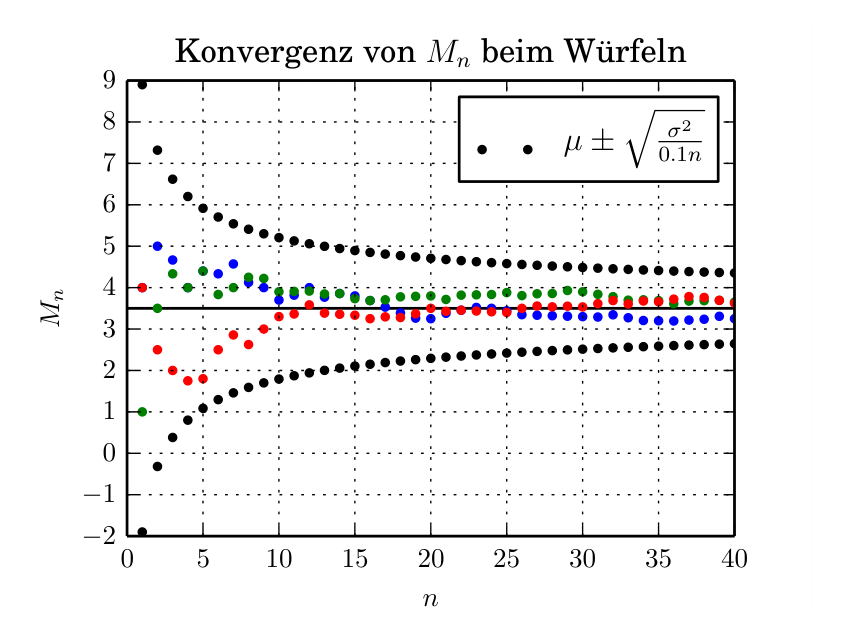
\includegraphics[scale=0.5]{assets/tschebyscheff.png}


\section{Central Limit Theorem}

Let $S_n \sim \text{Bin}(n,p)$ with a fixed $0 < p < 1$ and $q := 1-p$.

We define 
\[S^*_n = \frac{S_n - np}{\sqrt{npq}}\]
as the normalized binomial distribution, with expected value 0 and variance 1.

For all $a,b \in \mathbb{R}$ with $a < b$:
\[\lim_{n\to\infty}\mathbb{P}(a \leq S^*_n \leq b) = \int_{a}^{b} \varphi(x)\,dx\]
\[\lim_{n\to\infty}\mathbb{P}(S^*_n \leq b) = \int_{-\infty}^{b} \varphi(x)\,dx\]

where $\varphi$ is the Gaussian bell function (standard normal density):
\[\varphi(x) := \frac{1}{\sqrt{2\pi}}e^{-\frac{x^2}{2}}\]

Essentially, this states that when the normalized binomial distribution has infinitely large $n$, it closely resembles a continuous function. Therefore, to compute the cumulative distribution function, integration is sufficient.

\section{General Models}

\subsection{General Probability Space}
A probability space is a triple $(\Omega, \mathcal{A}, \mathbb{P})$ where:
\begin{itemize}
    \item $\Omega \neq \emptyset$ (sample space)
    \item $\mathcal{A}$ is a $\sigma$-algebra on $\Omega$ with:
    \begin{itemize}
        \item $\Omega \in \mathcal{A}$
        \item $A \in \mathcal{A} \Rightarrow \overline{A} := \Omega \setminus A \in \mathcal{A}$
    \end{itemize}
    \item $\mathbb{P}:\mathcal{A} \to [0,1]$ is a probability measure with:
    \begin{itemize}
        \item $\forall A \in \mathcal{A} : \mathbb{P}(A) \geq 0$
        \item $\mathbb{P}(\Omega) = 1$
    \end{itemize}
\end{itemize}

We define a \textbf{random variable} $X$ as a function $X: \Omega \to \mathbb{R}$ with the measurable property:
\[\{\omega \in \Omega : X(\omega) \leq x\} \in \mathcal{A}, \quad \forall x \in \mathbb{R}\]

\textit{Informally, this means that for any real number $x$, the set of all outcomes where the random variable $X$ takes a value less than or equal to $x$ must be an event we can assign a probability to (i.e., it must be in our $\sigma$-algebra $\mathcal{A}$).}

\subsubsection{Distribution Function}
\[F: \mathbb{R} \to [0,1]\]
\[F(x) := \mathbb{P}(X\leq x), \quad \forall x \in \mathbb{R}\]

Properties: $F$ is monotonically increasing and right-continuous, with $\lim_{x \to -\infty} F(x) = 0$ and $\lim_{x \to \infty} F(x) = 1$.

\subsubsection{Density Function}
For continuous probability spaces, the probability at any specific point is zero, so we use a different representation that describes the probability in an \textbf{area}.

\[f: \mathbb{R} \to \mathbb{R}_{\geq 0}\]

The total area under the density function equals 1, and it is tightly related to the distribution function:
\[F(x) = \int_{-\infty}^{x} f(t)\,dt\]

Expected value and variance:
\[\mathbb{E}(X) = \int_{-\infty}^{\infty}x \cdot f(x)\,dx\]
\[\mathbb{V}(X) = \int_{-\infty}^{\infty}(x - \mathbb{E}(X))^2 \cdot f(x)\,dx = \mathbb{E}\left[(X - \mathbb{E}(X))^2\right] = \sigma^2(X)\]


\subsection{Uniform Distribution}
A random variable is uniformly distributed, $X \sim \mathcal{U}(a,b)$, if:
\[f(x) := \begin{cases}
    \frac{1}{b-a} & x \in [a,b] \\
    0 & \text{otherwise}
\end{cases}\]

\[\mathbb{E}(X) = \frac{a+b}{2}\]
\[\mathbb{V}(X) = \frac{(b-a)^2}{12}\]


\subsection{Exponential Distribution}
A random variable is exponentially distributed with parameter $\lambda > 0$, denoted $X \sim \text{Exp}(\lambda)$, if:
\[f(x) := \begin{cases}
    0 & x \leq 0 \\
    \lambda e^{-\lambda x} & x > 0
\end{cases}\]

Distribution function:
\[F(x) := \begin{cases}
    0 & x \leq 0 \\
    1 - e^{-\lambda x} & x > 0 
\end{cases}\]

\[\mathbb{E}(X) = \frac{1}{\lambda}\]
\[\mathbb{V}(X) = \frac{1}{\lambda^2}\]

\subsection{Normal Distribution}
A random variable is normally distributed with parameters $\mu \in \mathbb{R}$ and $\sigma > 0$, denoted $X \sim \mathcal{N}(\mu,\sigma^2)$, if:

\[f(x) := \frac{1}{\sigma\sqrt{2\pi}} \exp\left(-\frac{(x-\mu)^2}{2\sigma^2}\right), \quad x\in \mathbb{R}\]

This somewhat resembles the binomial distribution. With parameters $(0,1)$, we obtain the Gaussian bell function.

We call $Z \sim \mathcal{N}(0,1)$ the \textbf{standard normal distribution}.

Also, we can transform: $X := \sigma \cdot Z + \mu$.

\[\mathbb{E}(X) = \mu\]
\[\mathbb{V}(X) = \sigma^2\]

\subsubsection{Quantiles}
Quantiles represent the $x$-coordinate that corresponds to a given percentage of the cumulative distribution function:

\[x_p = (F^X)^{-1}(p) = \sigma z_p + \mu\]

where $z_p$ is the $p$-quantile of the standard normal distribution.

\vspace{0.5em}
\noindent\textbf{Important $p$-quantiles for standard normal distribution:}

\begin{center}
\begin{tabular}{|c|c|c|c|c|c|c|}
    \hline
    $p$ & 50\% & 75\% & 90\% & 95\% & 97.5\% & 99\%\\
    \hline
    $z_p$ & 0.00 & 0.67 & 1.28 & 1.64 & 1.96 & 2.33\\ 
    \hline
\end{tabular}
\end{center}

\subsubsection{$k\sigma$-Ranges}
The inverse of quantiles: you specify a number $k$ corresponding to the width of the interval (in multiples of $\sigma$) in each direction from the mean, and you get the probability:
\[\mathbb{P}(\mu - k\sigma \leq X \leq \mu + k\sigma)\]

\subsection{Chi-Square Distribution}
Let $X_i, i = 1,\ldots,n$ be independent and identically distributed random variables following the standard normal distribution.

Then we call $Z = X_1^2 + \cdots + X_n^2$ \textbf{chi-square distributed} with $n$ degrees of freedom:

\[Z \sim \chi^2(n)\]
\[\mathbb{E}(Z) = n\]
\[\mathbb{V}(Z) = 2n\]


\subsubsection{Student's $t$-Distribution}
Let $X$ be standard normally distributed and $Z \sim \chi^2(n)$ be independent. Then
\[T = \frac{X}{\sqrt{Z/n}}\] 
is called \textbf{$t$-distributed} with $n$ degrees of freedom:

\[T \sim t(n)\]

\[\mathbb{E}(T) = 0, \quad (n \geq 2)\]
\[\mathbb{V}(T) = \frac{n}{n-2}, \quad (n \geq 3)\]


\subsubsection{Fisher's $F$-Distribution}

Let $X \sim \chi^2(m)$ and $Y \sim \chi^2(n)$ be independent. Then
\[Z = \frac{X/m}{Y/n}\] 
is \textbf{Fisher distributed} with $m$ and $n$ degrees of freedom:
\[Z \sim F(m,n)\]

\[\mathbb{E}(Z) = \frac{n}{n-2}, \quad n \geq 3\]
\[\mathbb{V}(Z) = \frac{2n^2(m+n-2)}{m(n-4)(n-2)^2}, \quad n \geq 5\]

\section{Multidimensional random variables}

\[\mathbb{P}^{(X,Y)}(\{(x,y)\}) = f(x,y) := \mathbb{P}(X = x, Y = y)\]

Note: $f(x,y)$ doesnt mean the function is continous, its just the discrete equivalent
\subsection{Marginal distribution (Randverteilung)}

\[f_X(x) = \mathbb{P}(X = x) = \sum_{j=1,2,..}f(x,y_j)\]
Analog für Y

\subsection{Conditional probability function}

\[f_X(x|y) = \frac{f(x,y)}{f_Y(y)}\]


\subsection{Total distribution function}

\[F(x,y) = \mathbb{P}( X \leq x, Y \leq y) = \sum_{x_i \leq x}\sum_{y_j \leq y}f(x_i,y_j)\]

\subsection{Marginal distribution function}

\[F_X(x) = \mathbb{P}(X \leq x) = F(x,\infty) = \sum_{x_i \leq x}\sum_{j = 1,2,...}f(x_i,y_j)\]

\subsection{Two dimensional continous random variables}

\subsubsection{Combined continous distribution and density function}

We call X,Y continous if there exists a two dimensional density function $f(x,y) \geq 0$ with

\[\mathbb{P}(a \leq X \leq b , c \leq Y \leq d) = \int_{a}^b\int_c^df(x,y)dy dx\]

\subsubsection{Marginal density}
\[f_X(x) = \int_{-\infty}^{\infty}f(x,y)dy\]

Total area at a point in x

\subsubsection{Combined Distribution Function}
\[F(x,y) = \int_{-\infty}^{x}\int_{-\infty}^{y}f(u,v)dvdu\]

\subsubsection{Conditional Density}
\[f_X(x|y) = \frac{f(x,y)}{f_Y(y)}\]


\subsubsection{Covariance}
It represents the degree to which two random variables vary together. A positive covariance indicates that the variables tend to move in the same direction, while a negative covariance indicates they tend to move in opposite directions. A covariance of zero suggests no linear relationship.
\[C(X,Y) = \mathbb{E}( (X - \mathbb{E}(X)) (Y - \mathbb{E}(Y)))\]


\subsubsection{Correlation}
It represents the standardized measure of linear association between two random variables, normalized to always lie between -1 and 1. A correlation of +1 indicates perfect positive linear relationship, -1 indicates perfect negative linear relationship, and 0 indicates no linear relationship. Unlike covariance, correlation is dimensionless and scale-independent.
\[r = r(X,Y) = \frac{C(X,Y)}{\sqrt{\mathbb{V}(X)\mathbb{V}(Y)}} = \frac{C(X,Y)}{\sigma_X\sigma_Y}\]
\subsection{2D Normal distribution}
 Complex formula hopefully it doesnt come in the exam

\newpage
\chapter{Statistik}

\section{Basic Concepts (translated)}
\begin{itemize}
    \item Statistische Einheit - Object that we analyze
    \item Population - Set of all those objects
    \item Stichprobe - Subset of the population we are actually analizing
    \item Merkmal - Characteristic we are checking
    \item Wert - Value of the characteristic for the object
    \item Kenngrö\ss e - Parameters
    \item Lagemaße - Dimensions
\end{itemize}


\section{Types of statistic}
\begin{itemize}
    \item Descriptive Statistic: Condensing information, no stochastic needed
    \item Explorative Statistic: Looking for structures and such in the data
    \item Inductive Statistic: Reach conclusions based on the data, uses stochastic and such
\end{itemize}

\section{Scales and characteristics}
\subsection{Characteristic types}
\begin{itemize}
    \item Discrete: Countable - Amount of workers in a company
    \item Continous: Values from an interval - Height of the workers
    \item Semi-Continous: Continous, but not continously measured - Age of workers
\end{itemize}
\subsection{Scales of characteristics}
\begin{itemize}
    \item Nominal Scale : Names - Categories
    \item Ordinal Scale: Ordered, but distance cant be measured
    \item Cardinal Scale: Ordered and distance can be measured
\end{itemize}

\section{Obtaining Data}
\subsection{No data yet}
Conduct an experiment
\subsection{Already have data}
Survey: collection of already existing data
\begin{enumerate}
    \item Survey for the data: primary statistics
    \item Survey based on existing (raw) data: secondary statistics
    \item Survey based on existing compressed/transformed data: tertiary statistics
\end{enumerate}

\subsubsection{Complete survey vs. sample survey}
One is harder to do, the other can cause bias/incorrect output data


\section{Univariate descriptive and explorative statistics}
Explorative and descriptive statistics are sometimes hard to distinguish, so they are treated together

Example: Measuring Clients per day

Objective: Describe the data, compress it, classify it and such


\subsection{Initial parameters: frequencies}

We have a feature X observed in n Objects

Raw data \[x_1,...,x_n \]

Classify by frequency
Observed values \[X:a_1,..,a_k | k \leq n\]
We define
\begin{itemize}
    \item $h(a_j) = h_j$ Absolute frequency
    \item $f(a_j) = f_j = \frac{h_j}{n}$ Relative frequency
    \item $h_1,..,h_k$ Absolute frequency distribution
    \item $f_1,..,f_k$ Relative frequency distribution
\end{itemize}

usually represented in a histogram

Usual rule of thumb
\[k = \lfloor \sqrt{n}\rfloor  \text{ for }n\leq 100\]
\[k = \lfloor10\log_{10}(n) \rfloor\]
\subsection{Graphical methods for univariate data}
\begin{itemize}
    \item Strichliste - Tally chart
    \item Stabdiagramm - Bar chart
    \item Säulen/-Balkendiagramm - Column/bar chart
    \item Histogramm - Histogram
    \item Kreisdiagramm - Pie chart
\end{itemize}
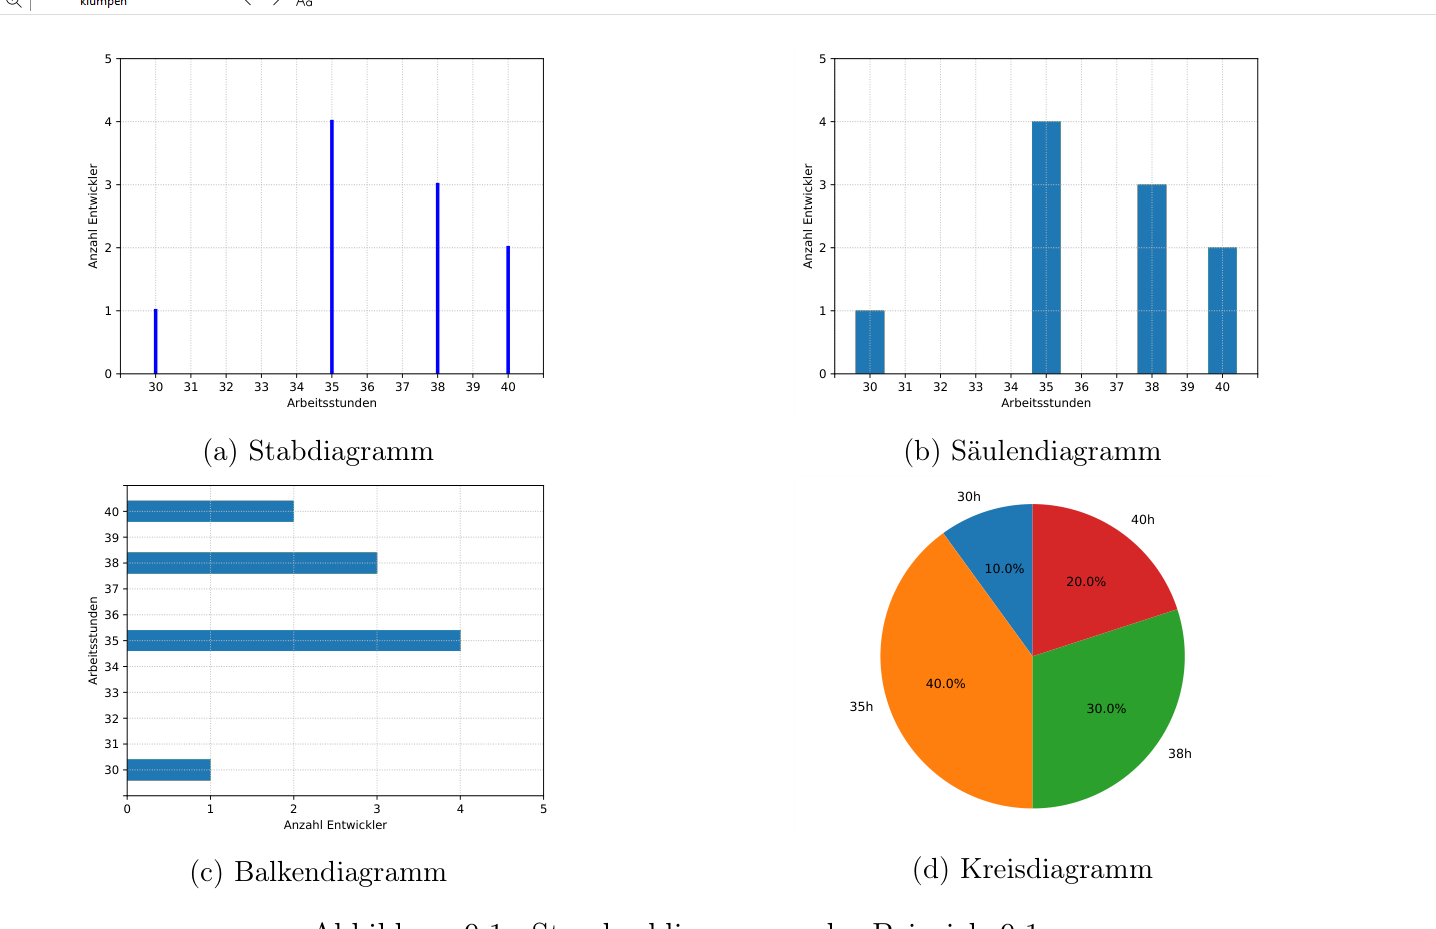
\includegraphics[scale=0.4]{assets/charts.png}

\subsection{Characterization of empirical distributions}
\subsubsection{Characterization over Form Parameters}

\begin{itemize}
    \item Amount of peaks: uni-,bi-,multimodal
    \item Steigung: linkssteil/rechtsschief
\end{itemize}

\subsubsection{Characterization over empirical distribution function}
\textbf{\underline{ONLY FOR ORDINAL SCALED DATA}}
\[H(x) = \sum_{i:a_i\leq x}h_j \text{ : absolute cumulative frequency distribution}\]
\[F(x) = \sum_{i:a_i\leq x}f_j \text{ : relative cumulative frequency distribution}\]
\[(\text{empirical distribution function})\]

\subsubsection{Characterization over center of distribution / location parameters}

Lagemaße := $L:\mathbb{R}^n \to \mathbb{R}$
\[L(x_1+a,...,x_n+a) = L(x_1,..,x_n) + a : \forall a,x_1,..,x_n \in \mathbb{R}\]
Describes the center of a distribution through a numerical value

Examples of center of the distribution
 \begin{itemize}
    \item arithmetic mean $\overline{x} = \frac{1}{n}\sum_{i=1}^nx_i$
    \item median $x_{med} = $ the one at the middle or the mean between the two in the middle
    \item mode: most freqeuent elemetn
    \item Geometrical mean: $x_{geom} = (x_1\cdot...\cdot x_n)^(\frac{1}{n})$ç
    \item Harmonical mean: $x_{harm} = \frac{1}{\frac{1}{n}\sum_{i=1}^n\frac{1}{x_j}}$
 \end{itemize}

 They can also be described as optimality equations

 \begin{itemize}
    \item $\overline{x}$ minimizes $Q(z,x_1,...,x_n) = \sum_{i=1}^n(x_i-z)^2$
    \item $x_{med}$ minimizes $Q(z,x_1,...,x_n) = \sum_{i=1}^n|x_i-z|$
    \item $x_{mod}$ minimizes $Q(z,x_1,...,x_n) = \sum_{i=1}^nI(x_i,z)$
    
    With $I(x_i,z)$ being the indicator function which equals 1 if $x_i \neq z$ and 0 otherwise

 \end{itemize}
\subsubsection{Characterization over dispersion measures}
Streuengsma\ss := $S:\mathbb{R}^n \to \mathbb{R}$

\[S(x_1+a,..,x_n+a) = S(x_1,..,x_n) \forall a,x_1,..,x_n \in \mathbb{R}\]

So somewhat like a number that represents the dispersion of the data, for example shifting the data by a doesnt affect it, same dispersion

\paragraph{Quantil (used later): } its like the inverse of the distribution function

\[x_p = F^{-1}(p)\]

Basically, its a \textbf{hypothetical} value that splits the data (ordered) in two, the left side has values $\leq x_p$ with at least $p$ of the data and the right side has values  $\geq x_p$with at least $1-p$

\textbf{NOT DISJOINT} 



Dispersion measures

\begin{itemize}
    \item Interquartilabstand (IQR): $d_Q = x_{0.75} -x_{0.25}$
\end{itemize}

We can have a 5-point summary to describe its dispersion
\[x_{min},x_{0.25},x_{med},x_{0.75},x_{max}\]


\paragraph{Graphical Representation - expanded box plot}
normal box plot is just the expanded version without the zaun


We draw a rectangle with right edge in $x_{0.75}$, left edge in $x_{0.25}$ and a like in $x_{med}$


Then we add two vertical lines in the values closest to the center such as
\[[z_u,z_o] = [x_{0.25} - 1.5d_Q, x_{0.75} +1.5d_Q]\] 

There shouldnt be to many points outside of fence, if any

\paragraph{Further dispersion measures}
\begin{itemize}
    \item Empirical Variance: $\tilde{s}^2 = \frac{1}{n}\sum (x_i - \overline{x})^2$
    \item Stichprobevarianz: $s^2 = \frac{1}{n-1}\sum(x_i-\overline{x})^2$
    \item Variationskoeffizient: $\tilde{v} = \frac{\tilde{s}}{\overline{x}}$
    \item Empirische standardabweichung: $\tilde{s} = \sqrt{\tilde{s}^2}$
\end{itemize}

The -1 in the Stichprobevarianz comes from that we already know the mean, so we lose one degreee of freedom, so that corrects it.


\paragraph{Transformation rule}: For a linear transformation $y = ax+b$

\[\tilde{s}_y^2 = a^2\tilde{s}_x^2 \text{ bzw } \tilde{s}_y = |a|\tilde{s}_x \]

This translates to that if data is multiplied by a and shifted by b, the effect on the variance of the shifting dissapears in the dispersion, and the multiplication is squared

The effect on the standardabweichung of shifting is also null and on the multiplication is scaled by $|a|$

\paragraph{Shift Theorem}: $\forall c\in \mathbb{R}$
\[\sum_{i=1}^n(x_i - c)^2 = \sum_{i=1}^n(x_i-\overline{x})^2 + n(\overline{x} - c)^2\]

If we subtitute for c = 0 and divide by n

\[\tilde{s}^2 = \left( \frac{1}{n}\sum_{i=1}^nx_i^2\right) - \overline{x}^2\]

This gives us a faster formula for empirical variance, and just generally divides the concept of

The total sum of squared distances to a point c can be divided into the spread around the arithmetical mean and the distance between the mean and c (n times)


\subsubsection{Characterization over form parameters}
\paragraph{Skewness (Schiefe) (moment coefficient)}
\[g_m = \frac{\frac{1}{n}\sum_{i=1}^n(x_i-\overline{x})^3}{\tilde{s}^3}\]
represents the symmetry of the data
\begin{itemize}
    \item 0 for symmetry, anything else deviates
\end{itemize}

\paragraph{ Curvature (Wölbung) (Fisher's curvature measure)}

\[\gamma = \frac{\frac{1}{n}\sum_{i=1}^n(x_i-\overline{x})^4}{\tilde{s}^4} - 3\]

Describes how strong the occupation of the central and peripherical areas of the data are
\begin{itemize}
    \item 0: resembles standard normal distribution
    \item > 0: spikier, extremes are populated
    \item < 0: flatter
\end{itemize}

\subsubsection{Characterization over Konzentrationsmaße}
\paragraph{Lorenz Curve: } Only for cardinalized , non negative characteristics. its a way to visualize concentration/ inequality
\[x_1\leq ... \leq x_n\]

The curve is the line that goes through the points $(0,0),(u_1,v_1),..,(u_n,v_n)$

With
\[u_j = \frac{j}{n}\]
\[v_j = \frac{\sum_{i=1}^jx_i}{\sum_{i=1}^nx_i}\]

Basically represents for a money and people statistic: Point (u,v) represents that u percentage of people own v percent of the money.

Always below the diagonal, pure diagonal means complete equality.

\paragraph{Gini-Coefficient}

\[G = \frac{\text{ surface between diagonal and lorenz curve}}{\text{ surface between diagonal and u-axis}} = \] 
\[ = 2 \cdot \text{ surface between diagonal and lorenz curve} = \]
\[ = \frac{2\sum_{i=1}^nix_i}{n\sum_{i=1}^nx_i} - \frac{n+1}{n}\]

We can also normalize it

\[G^*=\frac{G}{G_{max}} = \frac{n}{n-1}G \in [0,1]\]

Higher gini Coefficient means more unequal, if zero completely equal

\section{Multivariate descriptive and explorative statistics}
We are now looking at multiple characteristics per object

\subsection{2D Contingency Tables}
Way of representing the statistics for 2 variables

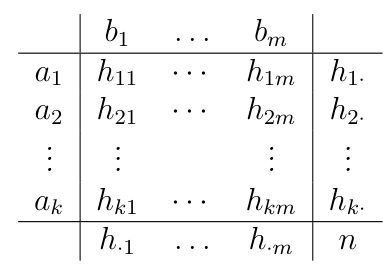
\includegraphics[scale=0.5]{assets/continencyTable.png}

Can also be done with relative frequencies instead


\paragraph{Conditioned relative probability distribution}

\[f_X(a_i|b_j) = \frac{h_{ij}}{h_{\cdot j}}\]

\subsection{Context analysis}
\subsubsection{$\chi^2 $ coefficient} 
Its defined through

\[\chi^2 = \sum_{i=1}^k\sum_{j=1}^m\frac{(h_{ij} - \tilde{h}_{ij})^2}{\tilde{h_{ij}}} = \sum_{i=1}^k\sum_{j=1}^m\frac{(h_{ij} - \frac{h_{i\cdot}h_{\cdot j}}{n})^2}{\frac{h_{i\cdot}h_{\cdot j}}{n}} \in [0,\infty)\]

This represents a discrepancy between $X$ and $Y$.
\begin{itemize}
    \item big value : X,Y are dependent on eachother
    \item small value : are independent
\end{itemize}

\subsubsection{Contingency coefficient} 

\[K = \sqrt{\frac{\chi^2}{n+\chi^2}} \in \left[0,\sqrt{\frac{M-1}{M}} \right] \text{ with } M = \min\{k,m\}\]

\subsubsection{Corrected contingency coefficient} 

\[K^* = \frac{K}{\sqrt{\frac{M-1}{M}}} \in [0,1]\]

Also represents how X and Y are related

\subsection{Analysis of Quantitative Characteristics}

\subsubsection{Empirical Correlation Coefficient}

For a sample size $(x_1,y_1),...,(x_n,y_n)$

\[r =  \frac{\sum_{i=1}^n (x_i - \overline{x})(y_i - \overline{y})}{\sqrt{\sum_{i=1}^n(x_i - \overline{x})^2} \sqrt{\sum_{i=1}^n(y_i - \overline{y})^2}}=\begin{cases}
    r > 0 & \text{ positive correlation}\\
    r < 0 & \text{ negative correlation}\\
    r = 0 & \text{ no correlation}
\end{cases}\]

\subsection{Linear Regression}
The idea is to model a set of data and 2 characteristics to a linear function $Y = f(X) + \epsilon$

with
\[f(X) = \alpha + \beta X\]
\[y_i = \alpha + \beta x_i + \epsilon_i\]

To get the most accurate function, we want to minimize each $\epsilon_i$, for that we have different methods

\subsubsection{Method of the smallest squares}
\[Q(\alpha,\beta)= \frac{1}{n}\sum_{i=1}^n\epsilon_i^2 = \frac{1}{n}\sum_{i=1}^n(y_i-(\alpha + \beta x_i))^2\]
We want to minimize Q, so we derive and equal to zero

after deriving (which we can do by hand)
\[\hat{\alpha} = \overline{y} - \hat{\beta}\overline{x} \]

\[\hat{\beta} = \frac{\tilde{s}_{x,y}}{\tilde{s}_x^2} \]

\subsubsection{Residual Analysis}
Measures how good a regression model is

We define $\hat{y}_i$ has the predicted value by the model
\begin{itemize}
    \item SQT (Sum of squares total): $\sum(y_i-\overline{y}_i)^2$ , how much the data varies around the 
    \item SQE (Sum of squares explained): $\sum(\hat{y}_i - \overline{y}_i)^2$ , how much the regression model explains the variation
    \item SQR (Sum of squares residual): $\sum(y_i - \hat{y}_i)^2$ measures the errors in the variation
\end{itemize}

\[SQT = SQE + SQR\]
\[\text{Total variability} = \text{explained variability} + \text{unexplained variability}\]

And we can look at how good the regression model is

\paragraph{Coefficient of determination - Bestimmtheitsmaß}
\[R^2 = \frac{SQE}{SQT}\]
What percentage of the variation is predicted
\begin{itemize}
    \item $R^2 = 1 $ Perfect fit with the model
    \item $R^2 = 0$ No relationship, regression model sucks
\end{itemize}

$R^2=0.8$ means  80\% of the variability in y is explained by x

\[R^2 = r_{xy}^2\]
r being the empirical correlation coefficient

\subsection{QQ-Plot (Quantil-Quantil Diagram)}

They are a diagramm where you plot the points $(x_p,y_p)$, representing the p-quantils of two characteristics

Then we can compare it with the analytical distribution

\section{Schätzprobleme (Estimating Problems)}
\end{document}